\documentclass[a4paper,12pt]{article} % тип документа

%  Русский язык
\usepackage[T2A]{fontenc}			% кодировка
\usepackage[utf8]{inputenc}			% кодировка исходного текста
\usepackage[english,russian]{babel}	% локализация и переносы

\usepackage{graphicx}               % импорт изображений
\usepackage{wrapfig}                % обтекаемые изображения
\graphicspath{{pictures/}}          % обращение к подкаталогу с изображениями
\usepackage[14pt]{extsizes}         % для того чтобы задать нестандартный 14-ый размер шрифта
\usepackage{amsfonts}               % буквы с двойными штрихами
\usepackage[warn]{mathtext}         % русский язык в формулах
\usepackage{indentfirst}            % indent first
\usepackage[margin = 25mm]{geometry}% отступы полей
\usepackage{amsmath}                % можно выводить фигурные скобочки -- делать системы уравнений
\usepackage[table,xcdraw]{xcolor}   % таблицы
\usepackage{amsmath,amsfonts,amssymb,amsthm,mathtools} % Математика
\usepackage{wasysym}                % ???
\usepackage{upgreek}                % ???  
\usepackage{caption}
\captionsetup{labelsep=period}
\usepackage{gensymb} % degree symbol

\begin{document}
	\begin{center}
		
		\textbf{НАЦИОНАЛЬНЫЙ ИССЛЕДОВАТЕЛЬСКИЙ УНИВЕРСИТЕТ \\ <<МОСКОВСКИЙ ФИЗИКО-ТЕХНИЧЕСКИЙ ИНСТИТУТ>>}
		\vspace{13ex}
		
		\textbf{Лабораторная работа 3.2.4(4.5) \\ <<Свободные колебания в электрическом контуре>> }
		\vspace{60ex}
		
		\normalsize{Овсянников Михаил Александрович \\ студент группы Б01-001\\ 2 курс ФРКТ\\}
	\end{center}
	
	\vfill 
	
	\begin{center}
		г. Долгопрудный\\ 
		2021 г.
	\end{center}
	
	\thispagestyle{empty} % выключаем отображение номера для этой страницы
	
	\newpage
	
\textbf{Цель работы:} исследование отклика колебательного контура на периодические внешние импульсы.

\textbf{В работе используются:} генератор импульсов, электронное реле, магазин сопротивлений, магазин емкостей, индуктивность, электронный осциллограф, универсальный мост.

\textbf{Экспериментальная установка.} На рис. 1 приведена схема для исследования свободных колебаний в контуре, содержащем постоянную индуктивность $L$ и переменные ёмкость $C$ и сопротивление $R$. Колебания наблюдаются на экране осциллографа.

\begin{figure}[h!]
	\centering
	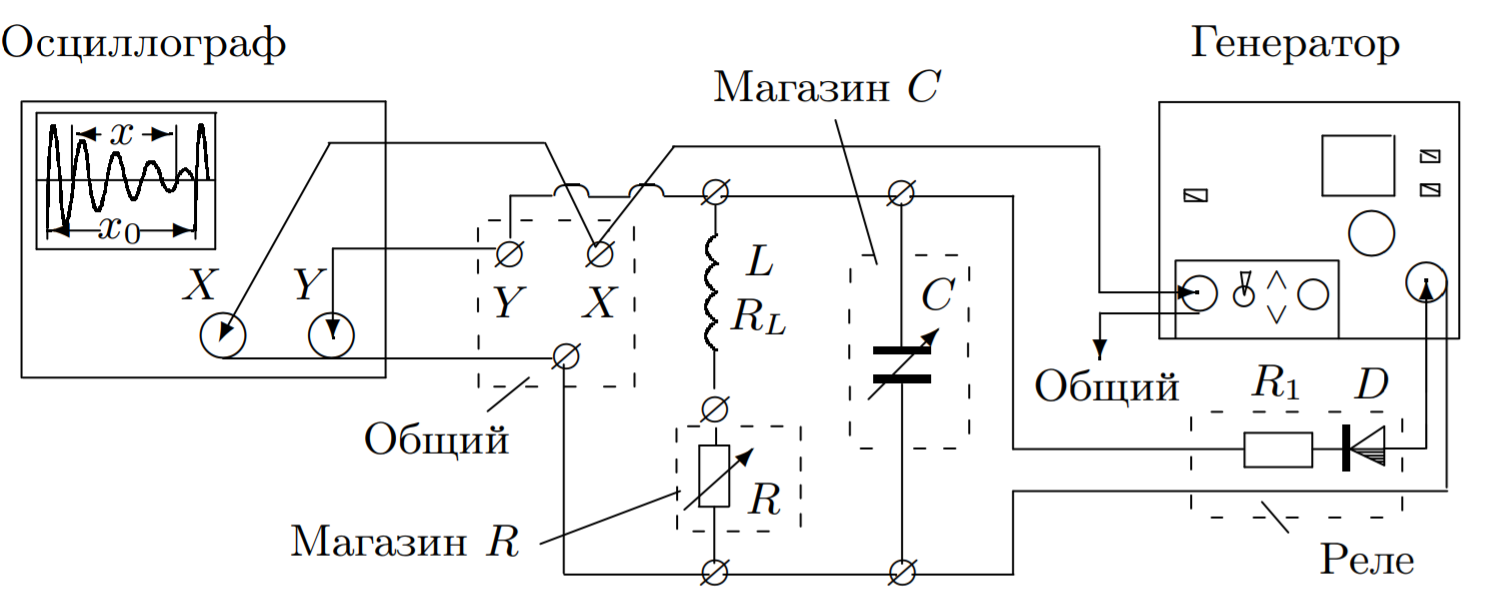
\includegraphics[scale=0.52]{Pictures/Установка.png}
	\caption*{Рис.1. Схема установки для исследования свободных колебаний}
\end{figure}


Выпишем все необходимые для работы расчетные формулы.

Период колебаний:
\begin{equation}
	T = 2\pi\sqrt{LC}
\end{equation}

Частота колебаний:
\begin{equation}
	\nu = \frac{1}{T} = \frac{1}{2\pi\sqrt{LC}}
\end{equation}

Логарифмический декремент затухания:
\begin{equation}
	\Theta = \ln{\frac{U_{k}}{U_{k+1}}} = \frac{1}{n}\ln{\frac{U_{k}}{U_{k+n}}}
\end{equation}

Критическое сопротивление:
\begin{equation}
	R_{\text{кр}} = 2\sqrt{\frac{L}{C}}
\end{equation}

Добротность:
\begin{equation}
	Q = 2\pi\frac{W}{\Delta W_{T}} = \frac{W}{\Delta W} = \frac{\pi}{\gamma T} = \frac{\omega_{0}L}{R} = \frac{1}{\omega_{0}CR} = \frac{1}{R}\sqrt{\frac{L}{C}}
\end{equation}


\newpage

\textbf{Ход работы:}

Соберем схему по рис.1.

При ненулевой нагрузке зафиксируем картины, которые показывает осциллограф для напряжения $U_c$ на конденсаторе и тока $I \thicksim \frac{dU_c}{dt}$ на нем.

\begin{figure}[h!]
	\centering
	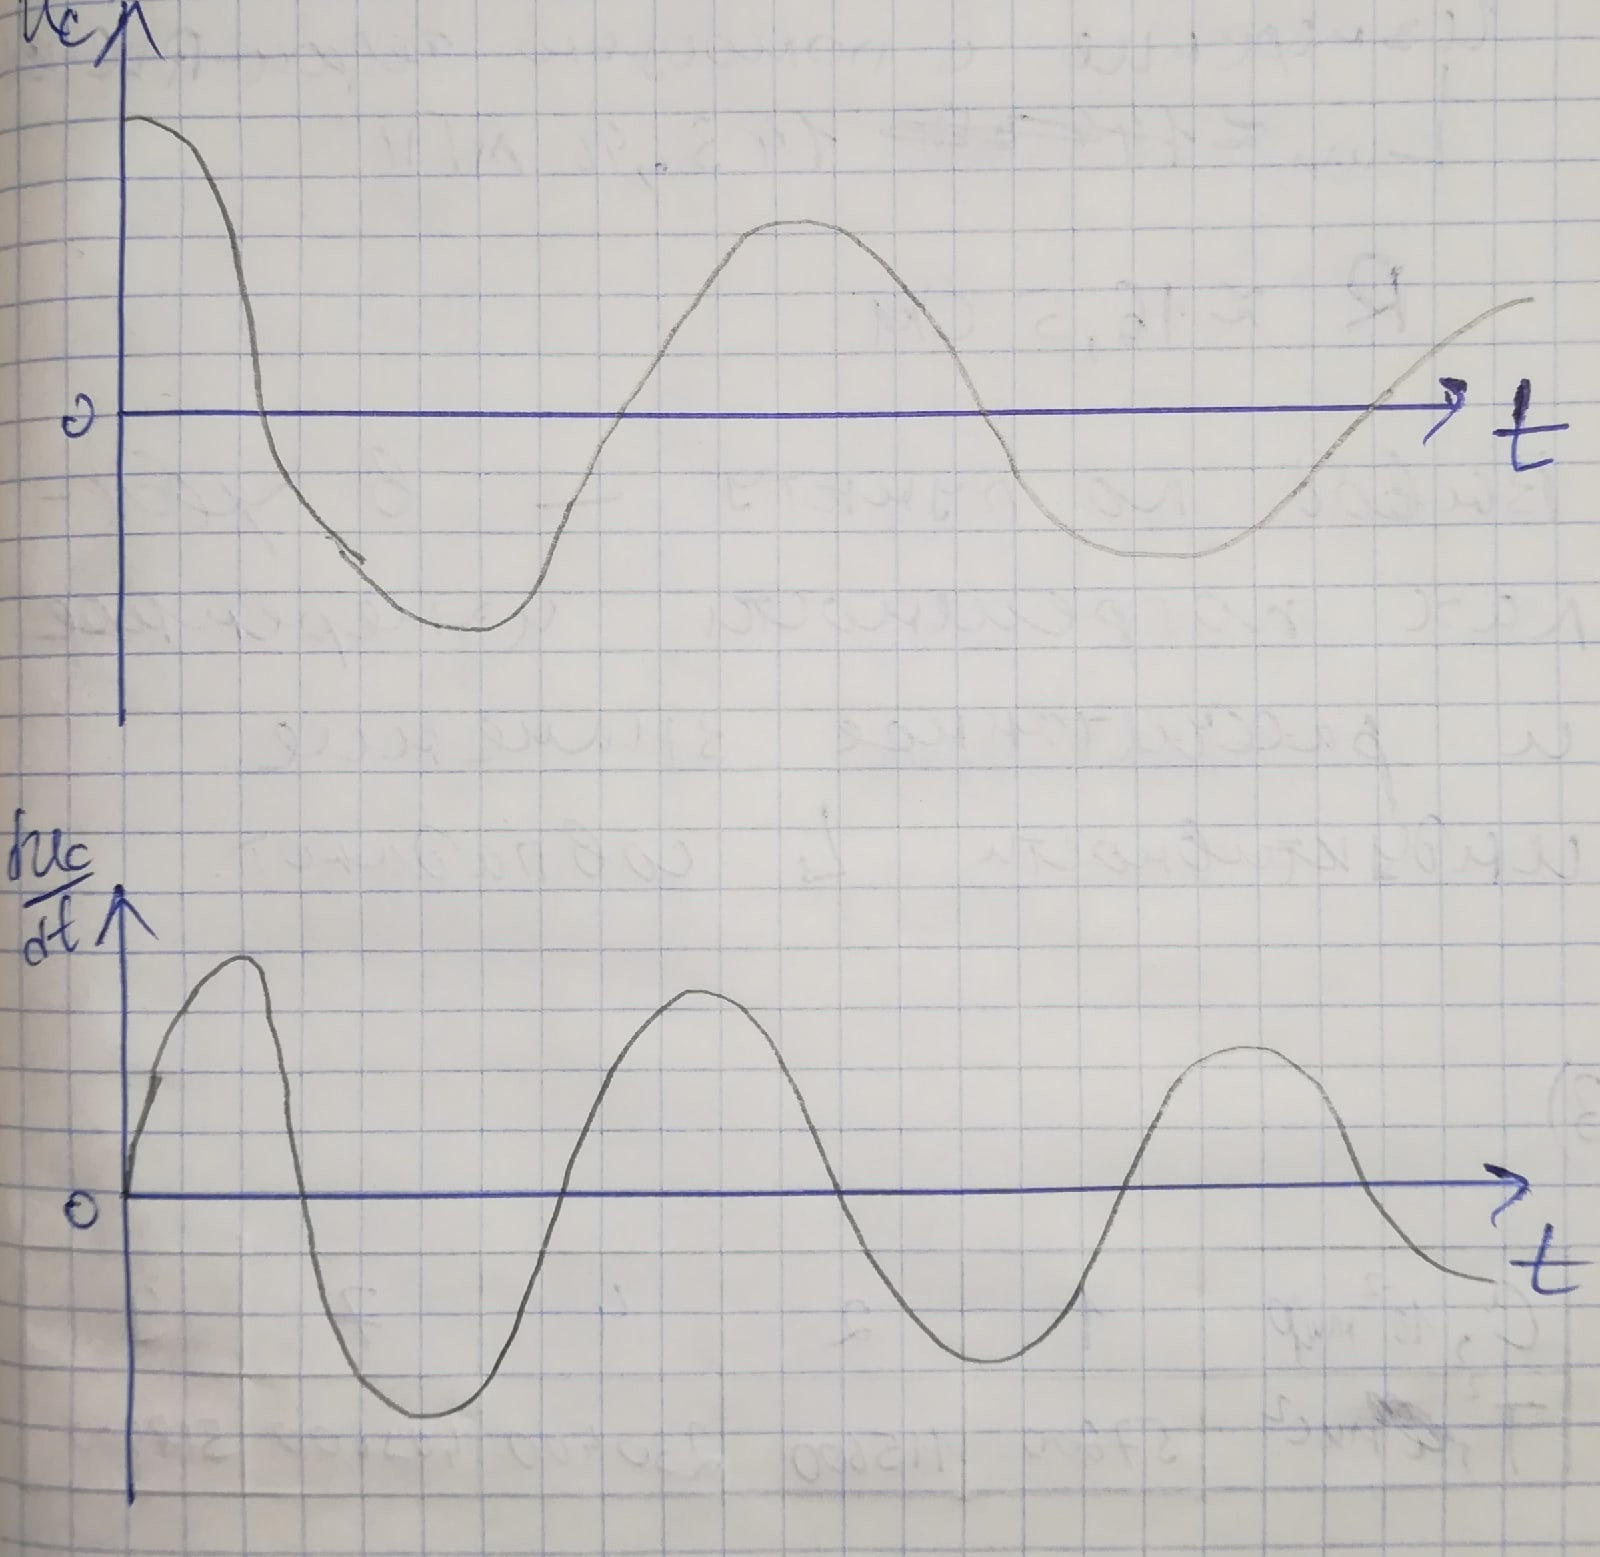
\includegraphics[scale=0.287]{Pictures/Конд.jpg}
\end{figure}

Из графиков видно, что в начальный момент времени заряд конденсатора максимален, а ток нулевой.
\vspace{5mm}

Выставим емкость конденсатора $C = 0,02$ мкФ $ = 2 \cdot 10^{-8}$ Ф.

По графикам из осциллографа найдем период $T = 340$ мкс.

Теперь по этим данным рассчитаем индуктивность катушки $L$:

\begin{equation*}
	T = 2\pi\sqrt{LC} \Longrightarrow L = \frac{T^2}{4\pi^2C} \approx 147 \text{ мГн}
\end{equation*}

Итак, $L_{\text{рассчетн}} = 147$ мГн.
\vspace{5mm}

Теперь измерим индуктивность катушки напрямую с помощью устройства ТЕТРОН-RLC-200:

$L_{\text{измер}} = 143$ мГн.

$R_{\text{катушки}} \approx 16,5$ Ом.

Как видим, в пределах погрешности измеренное и рассчитанное значения индуктивности $L$ совпадают.
\vspace{7mm}

Теперь измерим зависимость квадрата периода от емкости при нулевом внешнем сопротивлении:

\begin{table}[h!]
	\centering
	\begin{tabular}{|c|c|c|c|c|c|}
		\hline
		$C$, $10^{-2}$ мкФ    & 1    & 2     & 4     & 7     & 9     \\ \hline
		$T^2$, $10^3$ мкс$^2$ & 57,6 & 115,6 & 230,4 & 409,6 & 518,4 \\ \hline
	\end{tabular}
\end{table}

Построим график этой зависимости.

Используя метод наименьших квадратов получаем:

$T^2(C) = aC + b$,  где

$a = 57,92 \text{ }\frac{10^{-1} \text{с}^2}{\text{Ф}} \hspace{15mm} b = -0,10 \cdot 10^3$ мкс$^2$;

$\sigma_a = 0,12 \text{ }\frac{10^{-1} \text{с}^2}{\text{Ф}} \hspace{15mm} \sigma_b = 0,37 \cdot 10^3$ мкс$^2$.

\begin{figure}[h!]
	\centering
	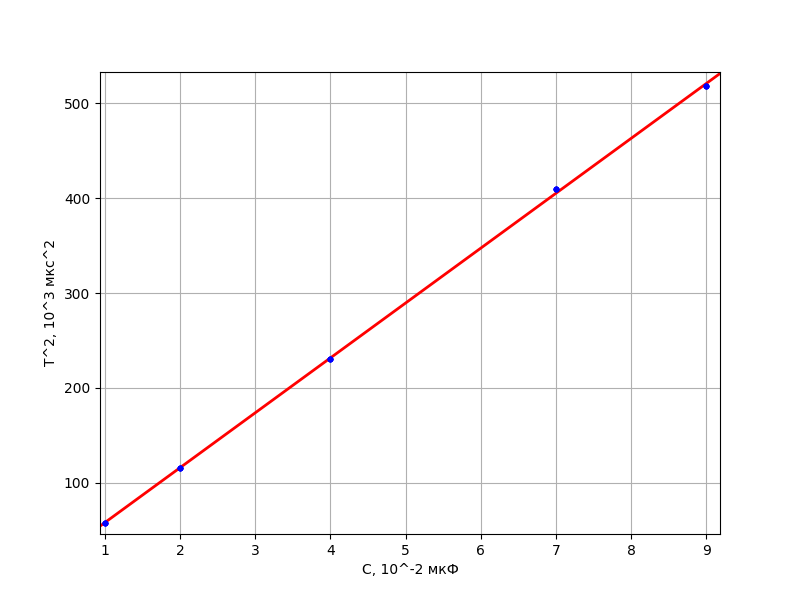
\includegraphics[scale=0.85]{Pictures/T^2(C).png}
\end{figure}

По графику видно, что точки хорошо ложатся на прямую.
\vspace{7mm}

Исследуем зависимость добротности системы $Q$ и логарифмического декремента затухания $\Theta$ от внешнего сопротивления $R_{\text{внеш}}$. Для этого будем изменять сопротивление в диапазоне от 0 до 15 Ом. На экране осциллографа выбираем два удаленных гребня, измеряем количество периодов $n$ между ними и отношение амплитуд $\frac{U_1}{U_n}$. Тогда $\Theta = \frac{1}{n}\ln\frac{U_1}{U_n}$, и $Q = \frac{\pi}{\Theta}$. Занесем все в таблицу:

\begin{table}[h!]
	\centering
	\begin{tabular}{|c|c|c|c|c|}
		\hline
		$R_{\text{внеш}}$, Ом & $n$ & $\frac{U_1}{U_n}$ & $\Theta$ & $Q$      \\ \hline
		0                     & 23  & 2                 & 0,030    & 104,60 \\ \hline
		2                     & 21  & 2                 & 0,033    & 95,15  \\ \hline
		4                     & 20  & 2                 & 0,034    & 92,35  \\ \hline
		6                     & 19  & 2                 & 0,036    & 87,22  \\ \hline
		8                     & 17  & 2                 & 0,041    & 76,59  \\ \hline
		10                    & 25  & 3                 & 0,044    & 71,36  \\ \hline
		12                    & 24  & 3                 & 0,046    & 68,26  \\ \hline
		15                    & 28  & 4                 & 0,049    & 64,08  \\ \hline
	\end{tabular}
\end{table}

Теперь построим график зависимости $\Theta(R_{\text{внеш}})$.

$\Theta = 2\pi \frac{R}{R_{\text{кр}}} = 2\pi \frac{R_{\text{внеш}}}{R_{\text{кр}}} + 2\pi\frac{R_{\text{внут}}}{R_{\text{кр}}}$

Опять же, используя МНК, получаем:

\noindent $\Theta = aR_{\text{внеш}} + b$, где

\noindent $a = 1,32 \cdot 10^{-3} $ Ом$^{-1}$ 

\noindent $b = 29,66 \cdot 10^{-3}$;

\noindent $\sigma_a = 0,07 \cdot 10^{-3} $ Ом$^{-1}$ 

\noindent $\sigma_b = 0,32 \cdot 10^{-3}$.
\vspace{7mm}

\noindent Получаем $R_{\text{кр}} = \frac{2\pi}{a} \approx 4760$ Ом $\thicksim 4800$  Ом.

\noindent $R_{\text{внут}} = \frac{bR_{\text{кр}}}{2\pi} \approx 22,47$ Ом.

\noindent Как видно из графика, точки неидеально, но все же ложатся на прямую.

\newpage

\begin{figure}[h!]
	\begin{center}
		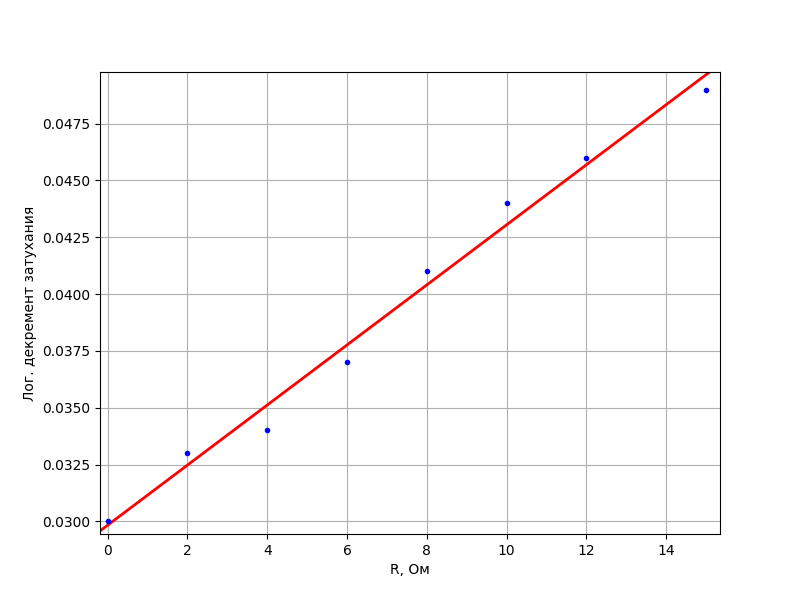
\includegraphics[scale=0.85]{Pictures/Q(R).png}
	\end{center}
\end{figure}

Произведем расчет и непосредственное измерение критического сопротивления $R_{\text{кр}}$.

Формула $R_{\text{кр}} = 2\sqrt{\frac{L}{C}}$.

Получаем $R_{\text{кр}} \approx 5366$ Ом $\thicksim 5400$ Ом.

По измерению получаем $R_{\text{кр}} \approx 4579$ Ом $\thicksim 4600$ Ом. Итак, все три значения (рассчетное, из графика и по эксперименту) достаточно близки друг к другу.

\newpage

\begin{figure}[h!]
	\centering
	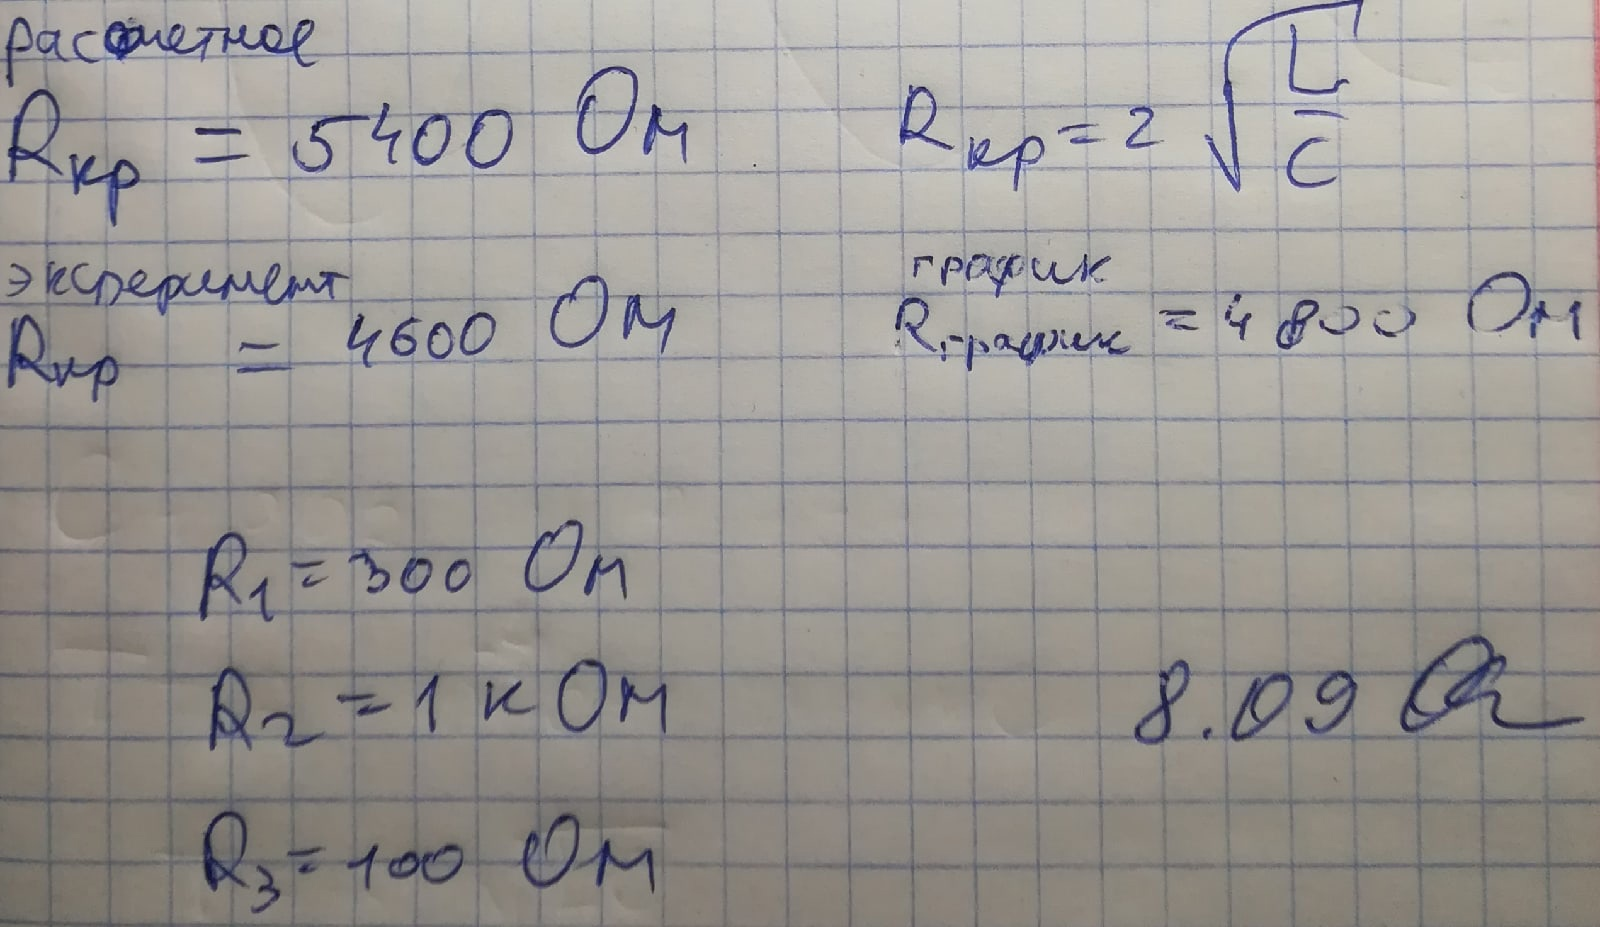
\includegraphics[scale=0.3]{Pictures/R.jpg}
\end{figure}

\vspace{7mm}

Посчитаем логарифмический декремент затухания $\Theta$ по фазовой диаграмме для трех разных значений сопротивления, указанных выше.

Способ тот же, что и при определении $\Theta$ по гребням волн, только амплитудой теперь является расстояние до центра.

1) $n = 6; \hspace{10mm} \frac{U_1}{U_n} = \frac{4,2}{0,4} = 10,5; \hspace{30mm} \Theta \approx 0,392$

\begin{figure}[h!]
	\centering
	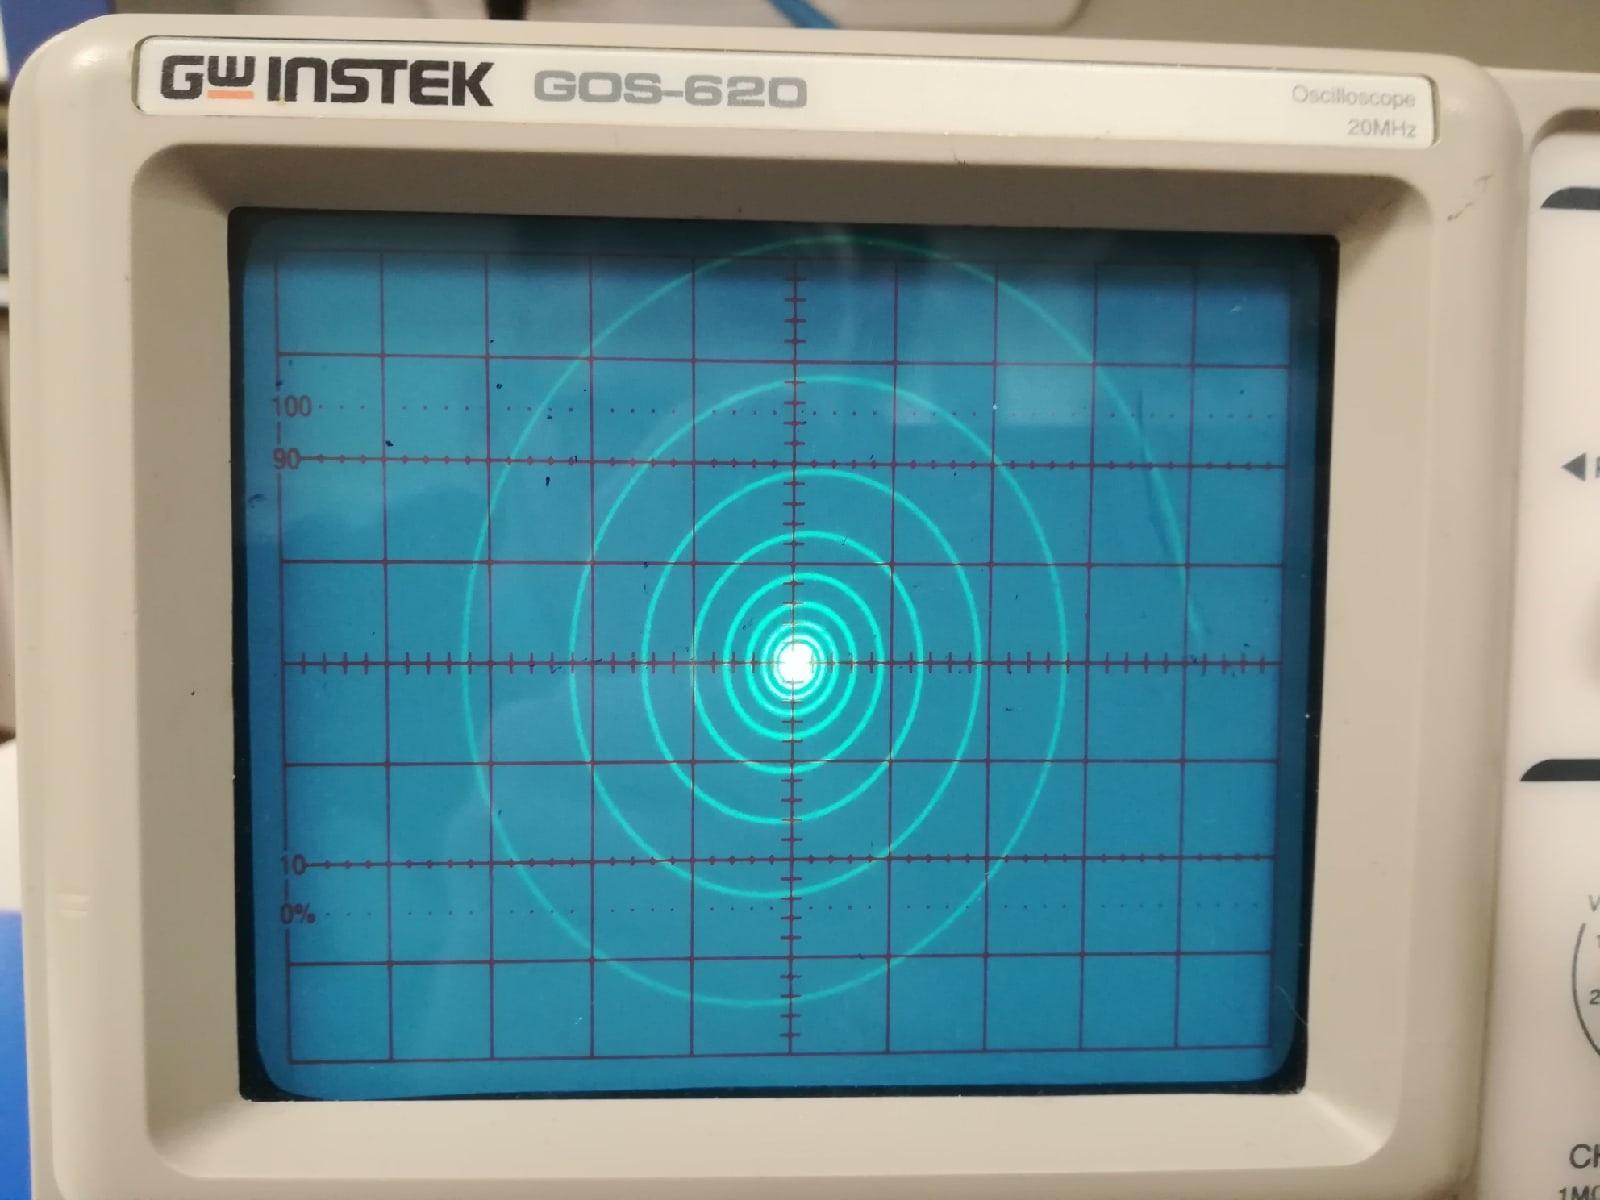
\includegraphics[scale=0.22]{Pictures/1.jpg}
\end{figure}

\newpage

2) $n = 2; \hspace{10mm} \frac{U_1}{U_n} = \frac{4,2}{0,4} = 10,5; \hspace{30mm} \Theta \approx 1,176$

\begin{figure}[h!]
	\centering
	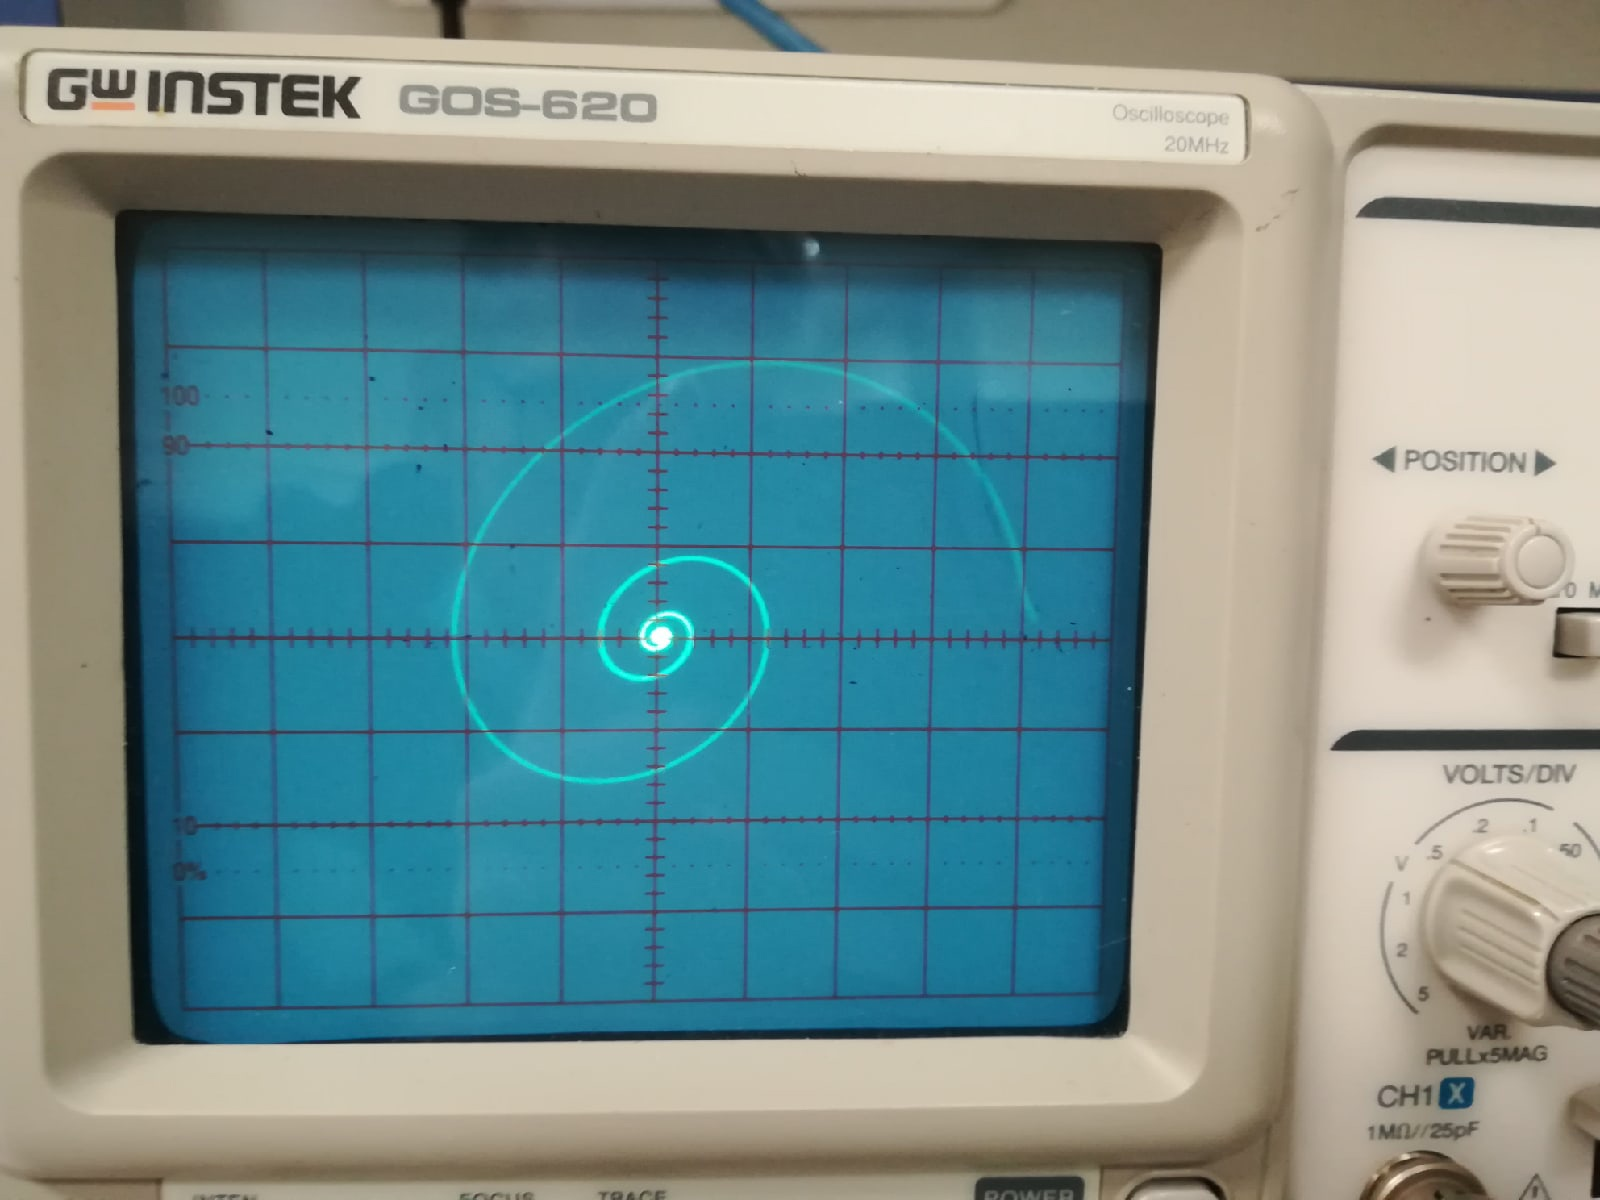
\includegraphics[scale=0.22]{Pictures/2.jpg}
\end{figure}

\vspace{15mm}

3) $n = 13; \hspace{10mm} \frac{U_1}{U_n} = \frac{4,2}{0,6} = 7,0; \hspace{30mm} \Theta \approx 0,150$

\begin{figure}[h!]
	\centering
	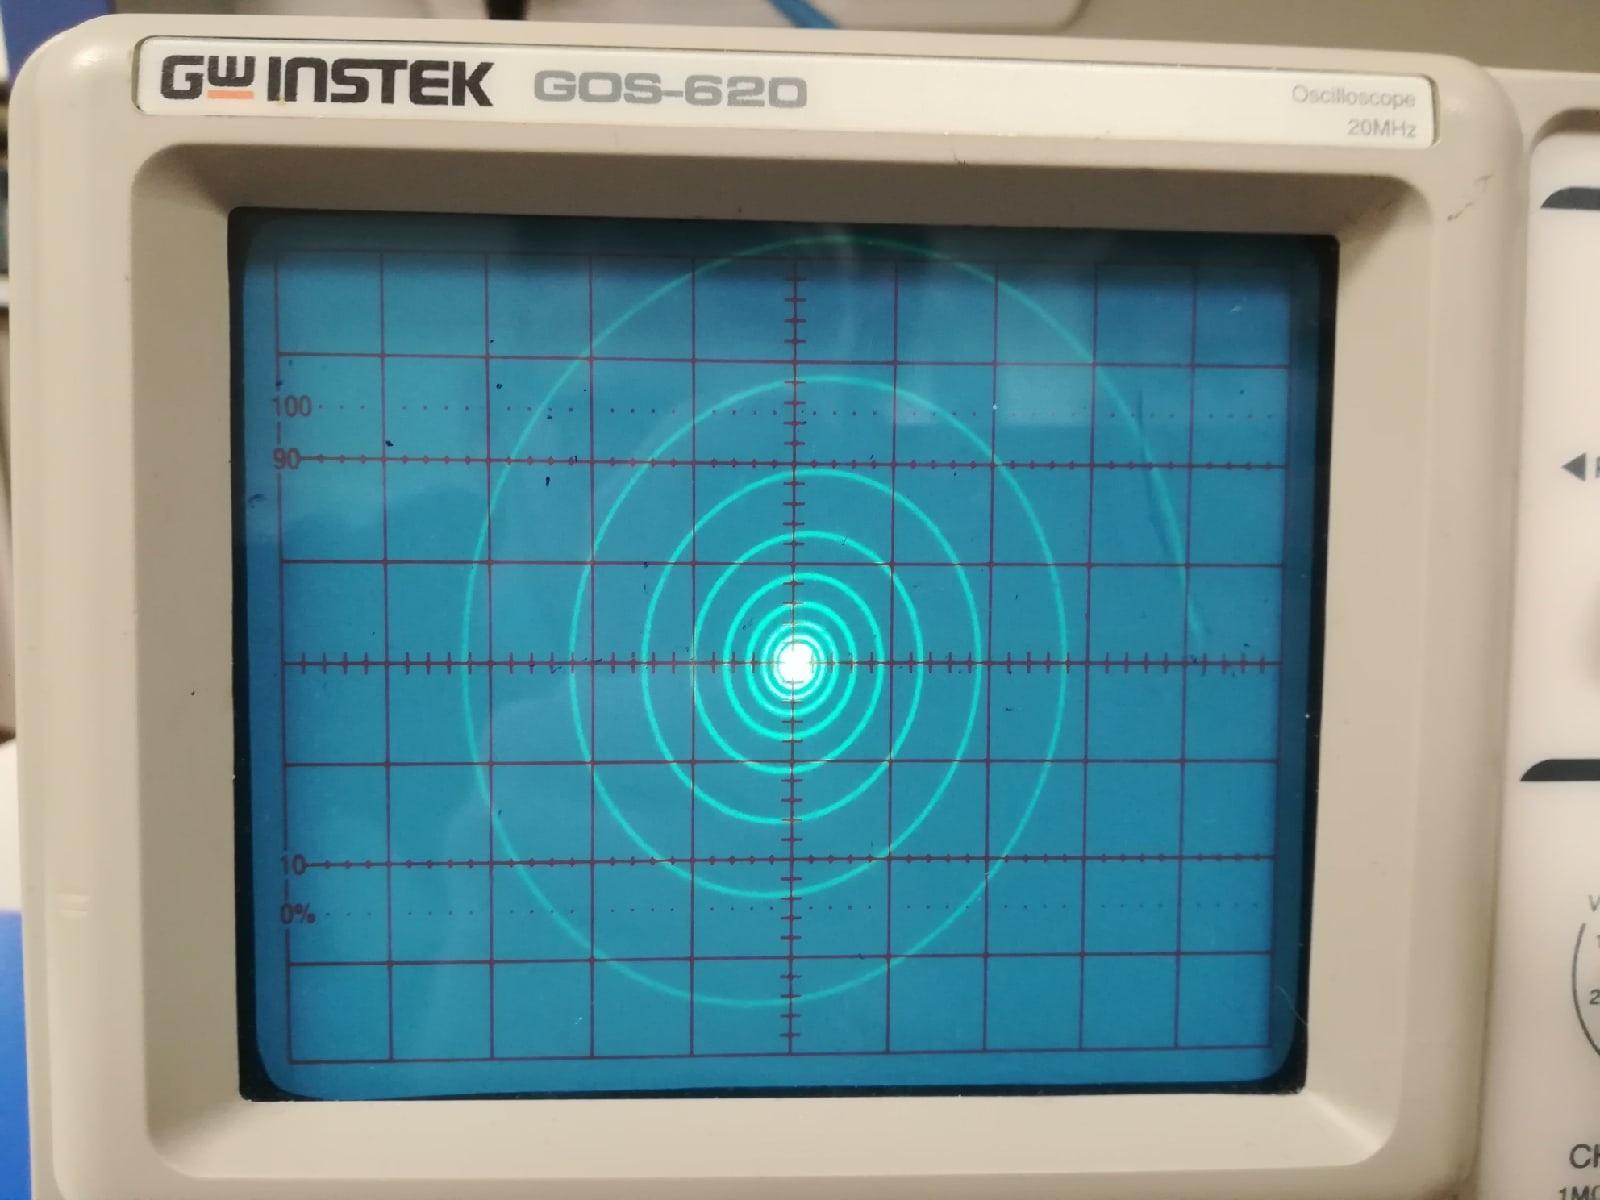
\includegraphics[scale=0.22]{Pictures/3.jpg}
\end{figure}

\newpage

\textbf{Вывод:} в данной работе было проведено исследование отклика колебательного контура на периодические внешние импульсы, проверена зависимость периода колебаний от емкости конденсатора, найдена индуктивность катушки $L = 143$ мГн, высчитано внутреннее сопротивление цепи $R_{\text{внут}} = 22,47$ Ом и исследована зависимость логарифмического декремента затухания колебаний от внешнего сопротивления цепи. Все ошибки связаны с погрешностью расчетов и неточностью измерений. 

\end{document}